\documentclass{article}

% packages
\usepackage{amsmath, amsthm, thmtools, amsfonts, amssymb, luacode, catchfile, tikzducks, hyperref, ifthen}
\ifcsname c@kobocompile\endcsname
	\usepackage[a5paper, total={1072pt, 1448pt}, margin=10pt, includeheadfoot]{geometry} % set page margins
\else
	\usepackage[a4paper, margin=50pt, includeheadfoot]{geometry}
\fi
\usepackage[shortlabels]{enumitem}
\usepackage[skip=3pt, indent=0pt]{parskip}

% language
\usepackage[bidi=basic, layout=tabular, provide=*]{babel}
\ifcsname c@english\endcsname
	\babelprovide[main, import]{english}
\else
	\babelprovide[main, import]{hebrew}
	\babelprovide{rl}
\fi
%\babelfont{rm}{Libertinus Serif}
\babelfont{rm}[Renderer=Harfbuzz]{Libertinus Serif}
\babelfont{sf}{Libertinus Sans}
\babelfont{tt}{Libertinus Mono}

% style
\AddToHook{cmd/section/before}{\clearpage}	% Add line break before section
\linespread{1.3}
\setcounter{secnumdepth}{0}		% Remove default number tags from sections, this won't do well with theorems
\AtBeginDocument{\setlength{\belowdisplayskip}{3pt}}
\AtBeginDocument{\setlength{\abovedisplayskip}{3pt}}
\graphicspath{ {../images/} }

% operators
\DeclareMathOperator\cis{cis}
\DeclareMathOperator\Sp{Sp}
\DeclareMathOperator\tr{tr}
\DeclareMathOperator\im{Im}
\DeclareMathOperator\re{Re}
\DeclareMathOperator\diag{diag}
\DeclareMathOperator*\lowlim{\underline{lim}}
\DeclareMathOperator*\uplim{\overline{lim}}
\DeclareMathOperator\rng{rng}
\DeclareMathOperator\Sym{Sym}
\DeclareMathOperator\Arg{Arg}
\DeclareMathOperator\Log{Log}
\DeclareMathOperator\dom{dom}
\DeclareMathOperator\supp{Supp}
\DeclareMathOperator\var{Var}
\DeclareMathOperator\cov{Cov}

% commands
%\renewcommand\qedsymbol{\textbf{מש''ל}}
%\renewcommand\qedsymbol{\fbox{\emoji{lizard}}}
\newcommand{\Aa}[0]{\mathcal{A}}
\newcommand{\Bb}[0]{\mathcal{B}}
\newcommand{\CC}[0]{\mathbb{C}}
\newcommand{\Cc}[0]{\mathcal{C}}
\newcommand{\EE}[0]{\mathbb{E}}
\newcommand{\FF}[0]{\mathbb{F}}
\newcommand{\Ff}[0]{\mathcal{F}}
\newcommand{\Ii}[0]{\mathcal{I}}
\newcommand{\Gg}[0]{\mathcal{G}}
\newcommand{\Ll}[0]{\mathcal{L}}
\newcommand{\Mm}[0]{\mathcal{M}}
\newcommand{\NN}[0]{\mathbb{N}}
\newcommand{\Nn}[0]{\mathcal{N}}
\newcommand{\PP}[0]{\mathbb{P}}
\newcommand{\Pp}[0]{\mathcal{P}}
\newcommand{\QQ}[0]{\mathbb{Q}}
\newcommand{\RR}[0]{\mathbb{R}}
\newcommand{\Rr}[0]{\mathcal{R}}
\newcommand{\Ss}[0]{\mathcal{S}}
\newcommand{\TT}[0]{\mathbb{T}}
\newcommand{\Uu}[0]{\mathcal{U}}
\newcommand{\Vv}[0]{\mathcal{V}}
\newcommand{\Ww}[0]{\mathcal{W}}
\newcommand{\ZZ}[0]{\mathbb{Z}}
\newcommand{\acts}[0]{\circlearrowright}
\newcommand{\explain}[2] {
	\begin{flalign*}
		 && \text{#2} && \text{#1}
	\end{flalign*}
}
\newcommand{\maketitleprint}[0]{ \begin{center}
	%\begin{tikzpicture}[scale=3]
	%	\duck[graduate=gray!20!black, tassel=red!70!black]
	%\end{tikzpicture}	
	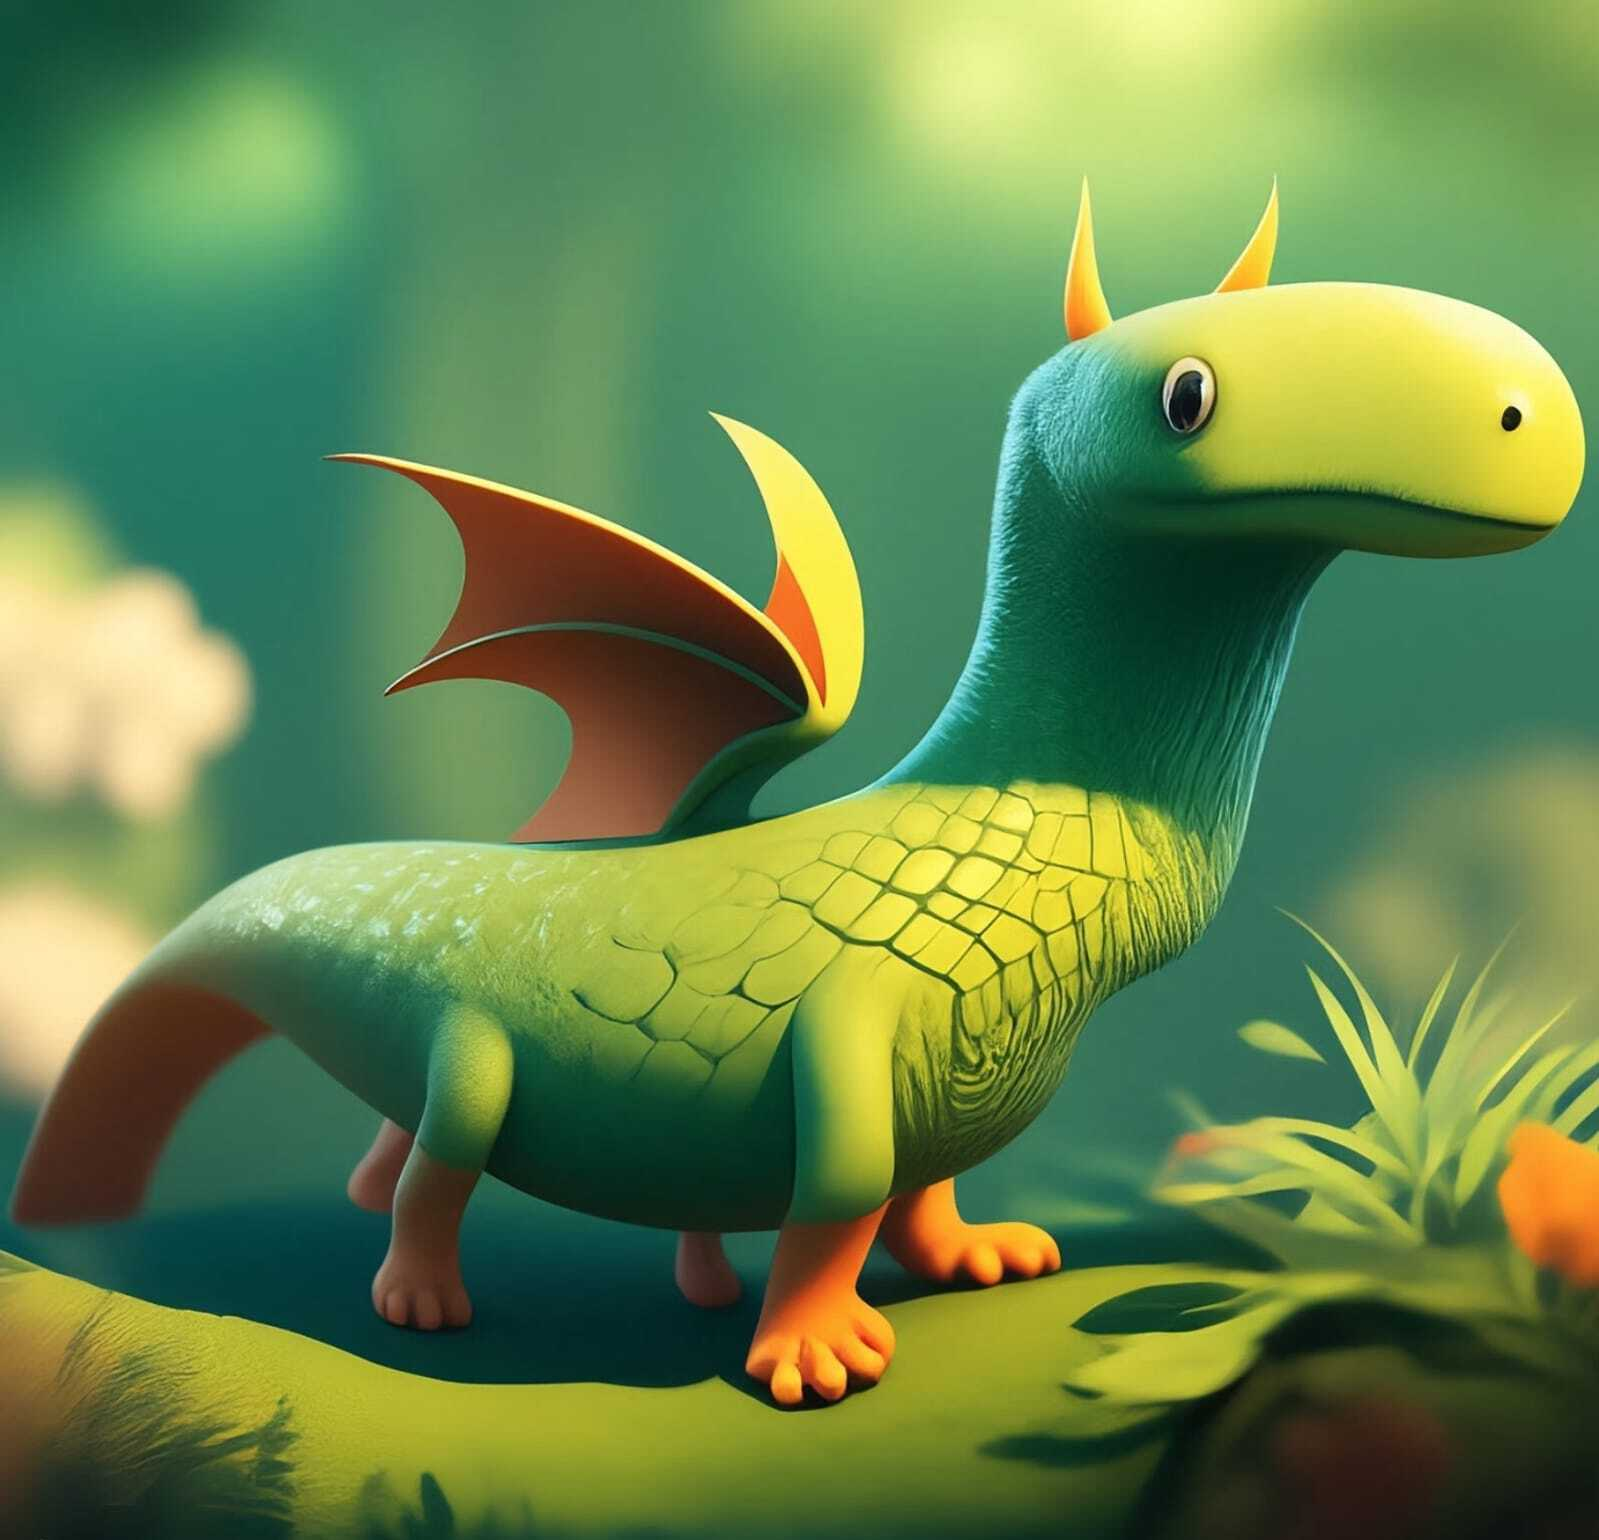
\includegraphics[width=6cm]{cover}
\end{center}
}

% theorem commands
\newtheoremstyle{c_remark}
	{}	% Space above
	{}	% Space below
	{}% Body font
	{}	% Indent amount
	{\bfseries}	% Theorem head font
	{}	% Punctuation after theorem head
	{.5em}	% Space after theorem head
	{\thmname{#1}\thmnumber{ #2}\thmnote{ \normalfont{\text{(#3)}}}}	% head content
\newtheoremstyle{c_definition}
	{3pt}	% Space above
	{3pt}	% Space below
	{}% Body font
	{}	% Indent amount
	{\bfseries}	% Theorem head font
	{}	% Punctuation after theorem head
	{.5em}	% Space after theorem head
	{\thmname{#1}\thmnumber{ #2}\thmnote{ \normalfont{\text{(#3)}}}}	% head content
\newtheoremstyle{c_plain}
	{3pt}	% Space above
	{3pt}	% Space below
	{\itshape}% Body font
	{}	% Indent amount
	{\bfseries}	% Theorem head font
	{}	% Punctuation after theorem head
	{.5em}	% Space after theorem head
	{\thmname{#1}\thmnumber{ #2}\thmnote{ \text{(#3)}}}	% head content

\ifcsname c@english\endcsname
	\theoremstyle{plain}
	\newtheorem{theorem}{Theorem}[section]
	\newtheorem{lemma}[theorem]{Lemma}
	\newtheorem{proposition}[theorem]{Proposition}
	\newtheorem*{proposition*}{Proposition}
	%\newtheorem{corollary}[theorem]{אין חלופה עברית}

	\theoremstyle{definition}
	\newtheorem{definition}[theorem]{Definition}
	\newtheorem*{definition*}{Definition}
	\newtheorem{example}{Example}[section]
	\newtheorem{exercise}{Exercise}[section]

	\theoremstyle{remark}
	\newtheorem*{remark}{Remark}
	\newtheorem*{solution}{Solution}
	\newtheorem{conclusion}[theorem]{Conclusion}
	\newtheorem{notation}[theorem]{Notation}
\else
	\theoremstyle{c_plain}
	\newtheorem{theorem}{משפט}[section]
	\newtheorem{lemma}[theorem]{למה}
	\newtheorem{proposition}[theorem]{טענה}
	\newtheorem*{proposition*}{טענה}
	%\newtheorem{corollary}[theorem]{אין חלופה עברית}

	\theoremstyle{c_definition}
	\newtheorem{definition}[theorem]{הגדרה}
	\newtheorem*{definition*}{הגדרה}
	\newtheorem{example}{דוגמה}[section]
	\newtheorem{exercise}{תרגיל}[section]

	\theoremstyle{c_remark}
	\newtheorem*{remark}{הערה}
	\newtheorem*{solution}{פתרון}
	\newtheorem{conclusion}[theorem]{מסקנה}
	\newtheorem{notation}[theorem]{סימון}
\fi

% Questions related commands
\newcounter{question}
\setcounter{question}{1}
\newcounter{sub_question}
\setcounter{sub_question}{1}

\ifcsname c@english\endcsname
	\newcommand{\question}[1][0]{
		\ifthenelse{#1 = 0}{}{\setcounter{question}{#1}}
		\section{Question \arabic{question}}
		\addtocounter{question}{1}
		\setcounter{sub_question}{1}
	}

	\newcommand{\subquestion}[1][0]{
		\ifthenelse{#1 = 0}{}{\setcounter{sub_question}{#1}}
		\subsection{Part \alph{sub_question}}
		\addtocounter{sub_question}{1}
	}
\else
	\newcommand{\question}[1][0]{
		\ifthenelse{#1 = 0}{}{\setcounter{question}{#1}}
		\section{שאלה \arabic{question}}
		\addtocounter{question}{1}
		\setcounter{sub_question}{1}
	}

	\newcommand{\subquestion}[1][0]{
		\ifthenelse{#1 = 0}{}{\setcounter{sub_question}{#1}}
		\subsection{סעיף \localecounter{letters.gershayim}{sub_question}}
		\addtocounter{sub_question}{1}
	}
\fi

% import lua and start of document
\directlua{common = require ('../common')}

\GetEnv{AUTHOR}

% headers
\author{\AUTHOR}
\date\today

\title{פתרון מטלה 01 --- מבוא ללוגיקה, 80423}

\begin{document}
\maketitle
\maketitleprint{}

\Question{}
יהי $T = (V, E)$ עץ כאשר $V$ סופית.

\Subquestion{}
נוכיח כי קיים מסלול ללא חזרות בין $v, u \in E$.
\begin{proof}
	יהי ${(v_n)}_{n = 1}^l$ מסלול סופי שמובטח שקיים מקשירות העץ כך ש־$v_1 = v, v_l = u$. \\*
	אילו אין חזרות סיימנו, לכן נניח שישנן חזרות, נבחר $0 \le i < j \le l$ כך ש־$v_i = v_j$.
	נבנה סדרה חדשה ${(v_n')}_{n = 1}^m$ על־ידי $v_k = v_k'$ לכל $0 \le k \le i$ ו־$v_k' = v_{k + j - i}$,
	זהו מסלול חדש בו אין את החזרה על $v_i$, והיא חוקית שכן ידוע כי $(v_{i - 1}, v_i), (v_j, v_{j + 1}) \in E$.
	נחזור על תהליך זה על $(v_n')$ שוב ושוב עד שנקבל מסלול ללא חזרות.
	נבחין כי אכן נקבל מסלול כזה, שכן כל מסלול הוא סופי, ולכן כמות החזרות אף היא סופית, וכמות החזרות לאחר התהליך קטנה ממש מכמות החזרות המקורית.
\end{proof}

\Subquestion{}
נוכיח כי אם $(v, u) \in E$ אז המסלול היחיד ללא חזרות ביניהם הוא $\langle v, w \rangle$.
\begin{proof}
	ידוע לנו כי קיים מסלול ללא חזרות בין שני הקודקודים, וברור כי $\langle v, u \rangle$ הוא מסלול כזה, עתה נוכיח את יחידותו. \\*
	יהי $\langle v_1, \dots, v_l \rangle$ מסלול נוסף ללא חזרות כך ש־$v_1 = v, v_l = u$.
	אילו $v_2 = u$ אז נקבל את המסלול שהגדרנו קודם, ולכן נניח כי $v_2 \ne u$.
	נבחין עתה כי ידוע שבמסלול אין מעגלים, לכן לא קיים $2 < i \le l$ כך ש־$v_i = v$, אך בעץ אין מעגלים ולכן נקבל ש־$G' = (V \setminus \{ v \}, E \setminus \{ v \} \times V)$ הוא גרף בעל שני רכיבי קשירות.
	יהי $G_1'$ רכיב הקשירות אשר מכיל את $v_2$, נוכל להסיק כי $u \notin G_1'$ אחרת נקבל סתירה להנחה ש־$v_2 \ne u$, ולכן נוכל לקבוע כי $\forall i, 0 \le i \le l \implies v_i \ne u$ וזו סתירה להגדרת מסלול זה.
	נסיק אם כן שקיים מסלול ללא חזרות יחיד והוא זה אשר ציינו.

	הוכחה נוספת והרבה יותר פשוטה:
	ידוע כי $\langle v, u \rangle$ מסלול ללא חזרות, נניח כי $\langle v = v_1, \dots, v_l = u \rangle$ מסלול נוסף כזה, אז $\langle v = v_1, \dots, v_l = u, v \rangle$ הוא מסלול ומעגל פשוט וזו סתירה להגדרת העץ,
	לכן מצאנו כי המסלול היחיד הוא אכן $\langle v, u \rangle$.
\end{proof}

\Subquestion{}
יהי מסלול ללא חזרות $\alpha = \langle v = v_0, \dots, v_l = u \rangle$ ונניח באינדוקציה תוך שימוש בסעיף הקודם כבסיס שלכל $2 \le k' < k$ יש מסלול ללא חזרות יחיד, ונוכיח כי גם המסלול הנתון הוא יחיד.
\begin{proof}
	נניח בשלילה כי קיים מסלול נוסף $\beta = \langle v = u_0, \dots, u_k = u \rangle$. \\*
	אילו קיים $0 < i < k$ כך ש־$v_i \in \beta$ אז מהנחת האינדוקציה נקבל כי קיים מסלול יחיד בין $v$ ל־$v_i$ ובין $v_i$ לבין $u$ ולכן $\alpha = \beta$ וקיבלנו סתירה לקיום מסלול נוסף. \\*
	נניח אם כן שאין $i$ כזה, דהינו המסלולים זרים מלבד בקצוות.
	נבנה מסלול חדש $\langle v = v_0, \dots, v_l = u = u_m, u_{m - 1}, \dots, u_0 = v \rangle$, נבחין כי במסלול זה אין חזרות מלבד בקצוות, והוא מתחיל ונגמר ב־$v$, דהינו מסלול זה הוא מעגל פשוט. \\*
	ידוע כי ב־$T$ אין מעגלים מהגדרתו כעץ ולכן קיבלנו סתירה, ואין מסלול נוסף המקיים את התנאים.
\end{proof}

\Subquestion{}
נוכיח כי $\le_T$ הוא יחס סדר חלקי.
\begin{proof}
	נגדיר $e \in V$ כגזע העץ, ונגדיר את $\le_T$ ביחס אליו, נוכיח כי הוא אכן סדר חלקי:
	\begin{itemize}
		\item רפלקסיביות: אם $\langle e = v_0, \dots, v_l = v \rangle$ מסלול, אז $v \in \langle v_i \rangle$ ולכן $v \le_T v$.
		\item אנטי־סימטריה: נניח כי $v \le_T u$ וגם $u \le_T v$,
			לכן קיים מסלול $\langle e = v_0, \dots, v_l = v \rangle$ וקיים מסלול $\langle e = u_0, \dots, v_m = u \rangle$ כך ש־$v_i = u, u_j = v$ עבור $0 \le i \le l, 0 \le j \le m$.
			אבל נקבל שכל מסלול מוכל בשני מהטענה שהוכחנו בסעיפים הקודמים, ולכן בפרט $i = j$ ו־$u = v$.
		\item טרנזיטיביות: נניח $u \le_T v, v \le_T w$, ולכן קיים מסלול בין $e$ לבין $w$ כך ש־$v$ מוכל בו, אבל יש מסלול יחיד גם בין $e$ ל־$v$ וידוע כי $u$ מוכל בו, לכן בפרט $u$ מוכל גם במסלול של $e$ ל־$w$ ומתקיים $u \le_T w$.
	\end{itemize}
\end{proof}

\Question{}
נוכיח כי אם $X \subseteq sent_L^+$ מקיימת לכל $\varphi \in X$ ש־$(\lnot \varphi) \in X$, וכן לכל $\square \in \mathcal{B}$ ולכל $\varphi, \psi \in X$ מתקיים $(\varphi \square \psi) \in X$ אז $sent_L^+ \subseteq X$.
\begin{proof}
	תהי קבוצה $X$ ונוכיח את הטענה באינדוקציה על אורך הסדרה.

	יהי $\varphi \in sent_L^+$ כך שקיימת סדרת יצירה $(\varphi_0)$ עבורה $\varphi = \varphi_0$, מהגדרת סדרות יצירה נוכל להסיק ישירות כי $\varphi_0 \in L$ ולכן $\varphi \in L$ ובהתאם להגדרת $X$ גם $\varphi \in X$.
	נשתמש בטענה זו כבסיס האינדוקציה.

	נניח את מעבר האינדוקציה, דהינו לכל $0 \le k < n$ אם $(\varphi_0, \dots, \varphi_k)$ אז $\varphi_k \in X$.
	יהי $\varphi \in sent_L^+$ כך שקיימת לו סדרת יצירה $(\psi_0, \dots, \psi_n)$ כך ש־$\varphi = \psi_n$.
	אילו $\varphi \in L$ אז ידוע כי $\varphi \in X$ וסיימנו.
	אם $\varphi = (\lnot \psi_k)$ עבור איזשהו $0 \le k < n$ אז נקבל $\psi_k \in X$ מהגדרת $X$ ולכן גם $\varphi \in X$.
	אם קיימים $0 \le k < l < n$ כך ש־$\varphi = (\psi_k \square \psi_l)$ אז נקבל כמובן מהנחת האינדוקציה $\psi_k, \psi_l \in X$ ובהתאם להגדרתה גם $\varphi \in X$.
	לכן נקבל כי $\varphi \in X$ תמיד והשלמנו את מהלך האינדוקציה.
\end{proof}

\Question{}
יהי $T = (V, E)$ חרוט בינארי סטנדרטי מיושר לשמאל, נגדיר $R \subseteq V$ קבוצת העלים שלו, ותהי $f : V \to \mathcal{B} \cup L \cup \{ \lnot \}$ המקיימת
\begin{itemize}
	\item $\forall t \in R, f(t) \in L$
	\item לכל $t \in T$ עם עוקב יחיד מתקיים $f(t) = \lnot$
	\item לכל $t \in T$ עם שני עוקבים מתקיים $f(t) \in \mathcal{B}$
\end{itemize}
נניח גם ש־$X$ קבוצה, $g : R \to X$ פונקציה, $\epsilon_\lnot : X \to X$ פונקציה ו־$\forall \square \in \mathcal{B}, \epsilon_\square : X \times X \to X$ פונקציות. \\*
נוכיח כי קיימת פונקציה יחידה $\tilde{g} : T \to X$ כך שמתקיים
\begin{itemize}
	\item $\forall t \in R, \tilde{g}(t) = g(t)$
	\item לכל $t \in T$ עם עוקב יחיד מתקיים $\tilde{g}(t) = \epsilon_\lnot(g(t \frown \langle 0 \rangle))$
	\item לכל $t \in T$ עם שני עוקבים מתקיים $\tilde{g}(t) = \epsilon_{f(t)}(\tilde{g}(t \frown \langle 0 \rangle), \tilde{g}(t \frown \langle 1 \rangle))$
\end{itemize}
\begin{proof}
	נוכיח שקיימת פונקציה כזו ושהיא אף יחידה באינדוקציה על גובה החרוט.

	נניח כי גובה החרוט הוא 1, דהינו $V = \{ s \}$ עבור $s \in {\{0, 1\}}^n$ כלשהו, אז נקבל $\tilde{g}(s) = g(s)$ בלבד, שכן $s \in R$.

	נניח כי הטענה נכונה לכל $0 \le k < n$, דהינו הפונקציה $\tilde{g}$ מוגדרת ויחידה עבור תת־חרוטים מגובה עד $n$, ונניח כי החרוט $T$ הוא בגובה $n$.
	עתה נבחין כי אם $s$ גזע החרוט, אז או שיש לו שני עוקבים או שיש לו עוקב יחיד, נבדוק את שני המקרים.
	אילו ל־$s$ יש עוקב יחיד $t = s \frown \langle 0 \rangle$, אז תת־העץ ששורשו הוא $t$ הוא עץ בגובה $n - 1$ ולכן $\tilde{g}(t)$ מוגדר ביחידות, ובהתאם נקבל $\tilde{g}(s) = \epsilon_\lnot(\tilde{g}(t))$ קיים ויחידי.
	אילו ל־$s$ שני עוקבים, $t_0 = s \frown \langle 0 \rangle, t_1 = s \frown \langle 1 \rangle$ אז נקבל באופן דומה כי גובה תת־העצים ששורשם $t_0, t_1$ הם לכל היותר $n - 1$.
	נוכל אם כן להסיק מהנחת האינדוקציה ש־$\tilde{g}(t_0), \tilde{g}(t_1)$ שניהם קיימים ביחידות, גם $f(s)$ מוגדר ביחידות, ולכן נוכל להסיק כי $\tilde{g}(s) = \epsilon_{f(t)}(\tilde{g}(t_0), \tilde{g}(t_1))$ בלבד.

	השלמנו את מהלך האינדוקציה ולכן לכל חרוט $T$ נקבל כי $\tilde{g}$ מוגדרת ויחידה.
\end{proof}

\end{document}
